%========================================================
% Permutation-Sorting Algorithms & Complexity (HSMW Uni Template)
% Beamer Presentation
%========================================================
\documentclass[aspectratio=169]{beamer}

\usetheme[
  hs,
  language=english,
  sectionslide
]{hsmw}

% ---------------- extra packages -----------------------
\usepackage{amsmath,amssymb}
\usepackage{animate}
\usepackage{array,booktabs,siunitx}   % tables
% Images handled by global draft option                 % figures
\usepackage{listings,xcolor}          % code blocks
\usepackage{hyperref}                 % hyperlinks
\usepackage[T1]{fontenc}
\usepackage{graphicx}

% ---------------- missing definitions ------------------
\newcolumntype{C}[1]{>{\centering\arraybackslash}p{#1}}

\lstdefinestyle{py}{
  language=Python,
  basicstyle=\ttfamily\small,
  keywordstyle=\color{blue!70!black},
  commentstyle=\color{gray}\itshape,
  stringstyle=\color{green!50!black},
  showstringspaces=false,
  frame=single,
  columns=fullflexible
}

% ---------------- header/footer -----------------------
\setbeamertemplate{footline}{%
  \leavevmode%
  \hbox{%
    \begin{beamercolorbox}[wd=.333\paperwidth,ht=2.25ex,dp=1ex,left]{author in head/foot}%
      \usebeamerfont{author in head/foot}\insertshortauthor~(\insertshortinstitute)
    \end{beamercolorbox}%
    \begin{beamercolorbox}[wd=.333\paperwidth,ht=2.25ex,dp=1ex,center]{title in head/foot}%
      \usebeamerfont{title in head/foot}\insertshorttitle
    \end{beamercolorbox}%
    \begin{beamercolorbox}[wd=.333\paperwidth,ht=2.25ex,dp=1ex,right]{date in head/foot}%
      \usebeamerfont{date in head/foot}\insertshortdate~\insertframenumber/\inserttotalframenumber
    \end{beamercolorbox}%
  }%
  \vskip0pt%
}

% -------------------------------------------------------
\title[Permutation-Sorting \& Complexity]{Permutation-Sorting Algorithms \& Complexity}
\subtitle[ISO-Date Experiments]{Practical ISO-Date String Experiments}
\author[Georgii Burdin]{Georgii Burdin}

\institute[Fakultät CB]{Fakultät CB}

\date[June 8, 2025]{June 8, 2025}

\begin{document}


% 2 Practical Application
\begin{frame}{Why and what for?}
  \vspace*{-1cm}
  \begin{itemize}
    \item Sorting is a fundamental operation in computer science, mathematics, and data analysis.
    \item Any sorting algorithm works by transforming an initial permutation of data into the sorted (identity) permutation.
    \item Understanding how algorithms handle permutations helps us analyze their efficiency and correctness.\\
  \textbf{Real-world uses of sorting algorithms:}
    \item Preparing data for time-series analysis and forecasting
    \item Applications in networking (packet reordering), cryptography, and more
    \item Organizing transaction or event logs by time.
    \item * I will use ISO-8601 date strings ("YYYY-MM-DD") as a concrete example for sorting. This reflects a common real-world need: sorting events by date (eg in reading logs of the system).

\end{itemize}
\end{frame}

\begin{frame}{What Is a Permutation?}
  \vspace*{-1cm}
  \textbf{Definition:}
    A \emph{permutation} of a finite set $S = \{1,2,\dots,n\}$ is a bijective function
      $\pi: S \to S$ \\
  \textbf{Notation:}
  \begin{itemize}
    \item A permutation can be written as a sequence $(\pi(1), \pi(2), \dots, \pi(n))$,
          meaning: $1$ goes to $\pi(1)$, $2$ goes to $\pi(2)$, etc.
    \item Example: For $n=4$, one possible permutation is $(3,1,4,2)$. This means:
      \begin{itemize}
        \item $1 \mapsto 3$
        \item $2 \mapsto 1$
        \item $3 \mapsto 4$
        \item $4 \mapsto 2$
      \end{itemize}
    \item The total number of permutations of $n$ objects is $n!$ (factorial).
  \medskip
  \end{itemize}
\end{frame}





% 6 Objectives & Setup
\begin{frame}{Experiment Summary}
  \begin{itemize}
    \item Implemented Bubble, Insertion, Merge, Quick and Heap in Python.
    \item Generated $n$ sequential ISO date strings from a random starting date.
    \item Shuffled the data into random, reversed, and already sorted orders.
    \item Measured runtime of 1000 random initialized datasets with \texttt{time.perf\_counter} and memory usage with \texttt{tracemalloc}.
    \item Compared and analyzed performance results for the five sorting algorithms.
    \item Made conclusions about which algorithms are fastest, slowest, and most efficient in terms of memory and time.
  \end{itemize}
\end{frame}


% 7 Algorithms Overview
\begin{frame}{Algorithms Overview}
  \vspace*{-0.5em}
  \scriptsize
  \begin{table}[ht]
    \centering
    \begin{tabular}{@{}l p{7cm} c c c@{}}
      \toprule
      \textbf{Algorithm} & \textbf{Core Idea} & \textbf{Best} & \textbf{Worst} & \textbf{Space} \\
      \midrule
      Bubble sort    & Swap adjacent out-of-order items               & $O(n)$        & $O(n^2)$      & $O(1)$       \\
      Insertion sort & Insert each element into sorted prefix         & $O(n)$        & $O(n^2)$      & $O(1)$       \\
      Merge sort     & Divide, sort, merge (stable)                   & $O(n\log n)$  & $O(n\log n)$  & $O(n)$       \\
      Quick sort     & Partition around pivot (in-place)              & $O(n\log n)$  & $O(n^2)$      & $O(\log n)$  \\
      Heap sort      & Build max-heap, extract max                    & $O(n\log n)$  & $O(n\log n)$  & $O(1)$       \\
      \bottomrule
    \end{tabular}
  \end{table}
\end{frame}


% 8 Bubble Sort: Idea & Math
\begin{frame}[fragile]{Bubble Sort}
\vspace*{-0.5cm}
  \begin{enumerate}
    \item \textbf{Scan:}
      Iterate through the list from the first element to the last.
    \item \textbf{Compare \& Swap:}
      For each adjacent pair $(a_j,a_{j+1})$, if $a_j > a_{j+1}$ swap them.
    \item \textbf{Repeat:}
      After each full pass the largest unsorted element “bubbles” to its correct position at the end. Continue passes until no swaps occur.
  \end{enumerate}
  \textbf{Example.}
\[
\begin{array}{l}
[4,3,2,1] \to
[3,4,2,1] \to
[3,2,4,1] \to
[3,2,1,4] \to \dots \to
[1,2,3,4]
\end{array}
\]
\end{frame}


\begin{frame}
\vspace*{-2cm}
  \centering
  % 8 fps, frames 000–060
  \animategraphics[autoplay,loop,width=.8\linewidth]{4}{graphs/bubbleFrame}{000}{060}
\end{frame}


% 10 Insertion Sort: Idea & Math
% ---------------- Insertion Sort ------------------------------------
\begin{frame}{Insertion Sort Step-by-Step}
\setlength{\leftmargini}{1.2em}
\setlength{\itemsep}{0.2em}
\begin{itemize}
  \item[\textcolor{blue}{\bfseries 1.}] \textbf{Pick the key} — the first item in the \emph{unsorted} tail.
  \item[\textcolor{blue}{\bfseries 2.}] \textbf{Shift larger items right} until you reach the key’s sorted position.
  \item[\textcolor{blue}{\bfseries 3.}] \textbf{Drop the key} into that gap. The sorted prefix is now one element longer.
\end{itemize}

\vspace{1ex}
\textbf{Example — ISO dates}
\scriptsize
\begin{tabular}{rlp{6cm}}
Init: & {[05, 02, 04, 01, 03]} & (start: first element is the 1-item sorted prefix) \\
1: & {[02, 05, 04, 01, 03]} & Key = 02; shift 05 right, insert 02 \\
2: & {[02, 04, 05, 01, 03]} & Key = 04; shift 05, insert 04 \\
3: & {[01, 02, 04, 05, 03]} & Key = 01; shift 05, 04, 02, insert 01 \\
4: & {[01, 02, 03, 04, 05]} & Key = 03; shift 05, 04, insert 03 (sorted) \\
\end{tabular}

\vspace{0.5ex}
{\footnotesize where 05 = 2025-06-05, 02 = 2025-06-02, etc.}
\end{frame}

\begin{frame}
\vspace*{-2cm}
  \centering
  % 8 fps, frames 000–060
  \animategraphics[autoplay,loop,width=.8\linewidth]{4}{graphs/insertionFrame}{000}{060}
\end{frame}


% 12 Merge Sort: Idea & Math
\begin{frame}[fragile]{Merge Sort}
\vspace*{-1.5cm}
  \begin{enumerate}
    \item \textbf{Divide:}
      Recursively split the list into halves until sublists of size $1$ remain.
    \item \textbf{Merge:}
      Repeatedly merge two sorted sublists into a single sorted list:
      \begin{itemize}
        \item Compare the smallest elements of each sublist,
        \item Copy the smaller element into the output buffer,
        \item Continue until all elements from both sublists are merged.
      \end{itemize}
    \item \textbf{Copy:}
      Copy the merged buffer back to the original list segment.
  \end{enumerate}
\textbf{Example.}
    \begin{aligned}
      &[\texttt{"2025-06-04"},\ \texttt{"2025-06-01"},\ \texttt{"2025-06-03"},\ \texttt{"2025-06-02"}] \\
      \to\ &[\texttt{"2025-06-04"},\ \texttt{"2025-06-01"}] + [\texttt{"2025-06-03"},\ \texttt{"2025-06-02"}] \\
      \to\ &[\texttt{"2025-06-01"},\ \texttt{"2025-06-04"}] + [\texttt{"2025-06-02"},\ \texttt{"2025-06-03"}] \\
      \to\ &[\texttt{"2025-06-01"},\ \texttt{"2025-06-02"},\ \texttt{"2025-06-03"},\ \texttt{"2025-06-04"}]
    \end{aligned}
\\
\end{frame}

\begin{frame}[fragile]{Merge Sort}
\vspace*{-2cm}
  \centering
  % 8 fps, frames 000–060
  \animategraphics[autoplay,loop,width=.8\linewidth]{2}{graphs/mergeFrame}{000}{060}

\end{frame}

% 14 Quick Sort: Idea & Math
\begin{frame}{Quick Sort}
  \textbf{Algorithm steps:}
  \begin{enumerate}
    \item \textbf{Choose a pivot:}
      Select an element from the array (e.g., first, last, or random).
    \item \textbf{Partition:}
      Rearrange elements so that:
      \begin{itemize}
        \item All elements $\leq$ pivot are moved to the left of the pivot,
        \item All elements $>$ pivot are moved to the right.
      \end{itemize}
    \item \textbf{Recursively sort:}
      Apply the same process to the left and right subarrays (excluding the pivot, which is now in its final position).
    \item \textbf{Base case:}
      Arrays of length $0$ or $1$ are already sorted.
  \end{enumerate}
  \medskip
\textbf{Example (pivot = 5).}
\[
6,2,9,4,8,\boxed{5}
\to 2,4,\boxed{5},9,8,6
\;(\text{then iteratively sort left and right subsets})
\]
\end{frame}

% 15 Quick Sort Animation
\begin{frame}[fragile]{Quick Sort}

\vspace*{-2cm}
  \centering
  % 2 fps, frames 000–060
  \animategraphics[autoplay,loop,width=.8\linewidth]{2}{graphs/quickFrame}{000}{026}
\end{frame}

% 16 Heap Sort: Idea & Math
\begin{frame}{Heap Sort:}
  \textbf{Algorithm steps:}
  \begin{enumerate}
    \item \textbf{Build a max-heap:}
      Transform the array into a max-heap, where each parent node is greater than or equal to its children.
    \item \textbf{Sort:}
      \begin{itemize}
        \item Swap the first element (the maximum) with the last element of the heap.
        \item Reduce the heap size by one (ignore the last sorted element).
        \item Restore the heap property (“sift down” the new root as needed).
        \item Repeat until the heap size is $1$.
      \end{itemize}
    \item \textbf{Result:} The array is now sorted in-place.
  \end{enumerate}\\

  \[
  \begin{aligned}
    &[\texttt{"2025-06-05"},\ \texttt{"2025-06-02"},\ \texttt{"2025-06-04"},\ \texttt{"2025-06-01"},\ \texttt{"2025-06-03"}]\\
    \to\ &[ \texttt{"2025-06-03"},\ \texttt{"2025-06-02"},\ \texttt{"2025-06-01"},\ \texttt{"2025-06-04"},\ \texttt{"2025-06-05"}]\\
    \to\ &[ \texttt{"2025-06-01"},\ \texttt{"2025-06-02"},\ \texttt{"2025-06-03"},\ \texttt{"2025-06-04"},\ \texttt{"2025-06-05"}]
  \end{aligned}
\]
\end{frame}

\begin{frame}{Heap Sort: Step by Step}
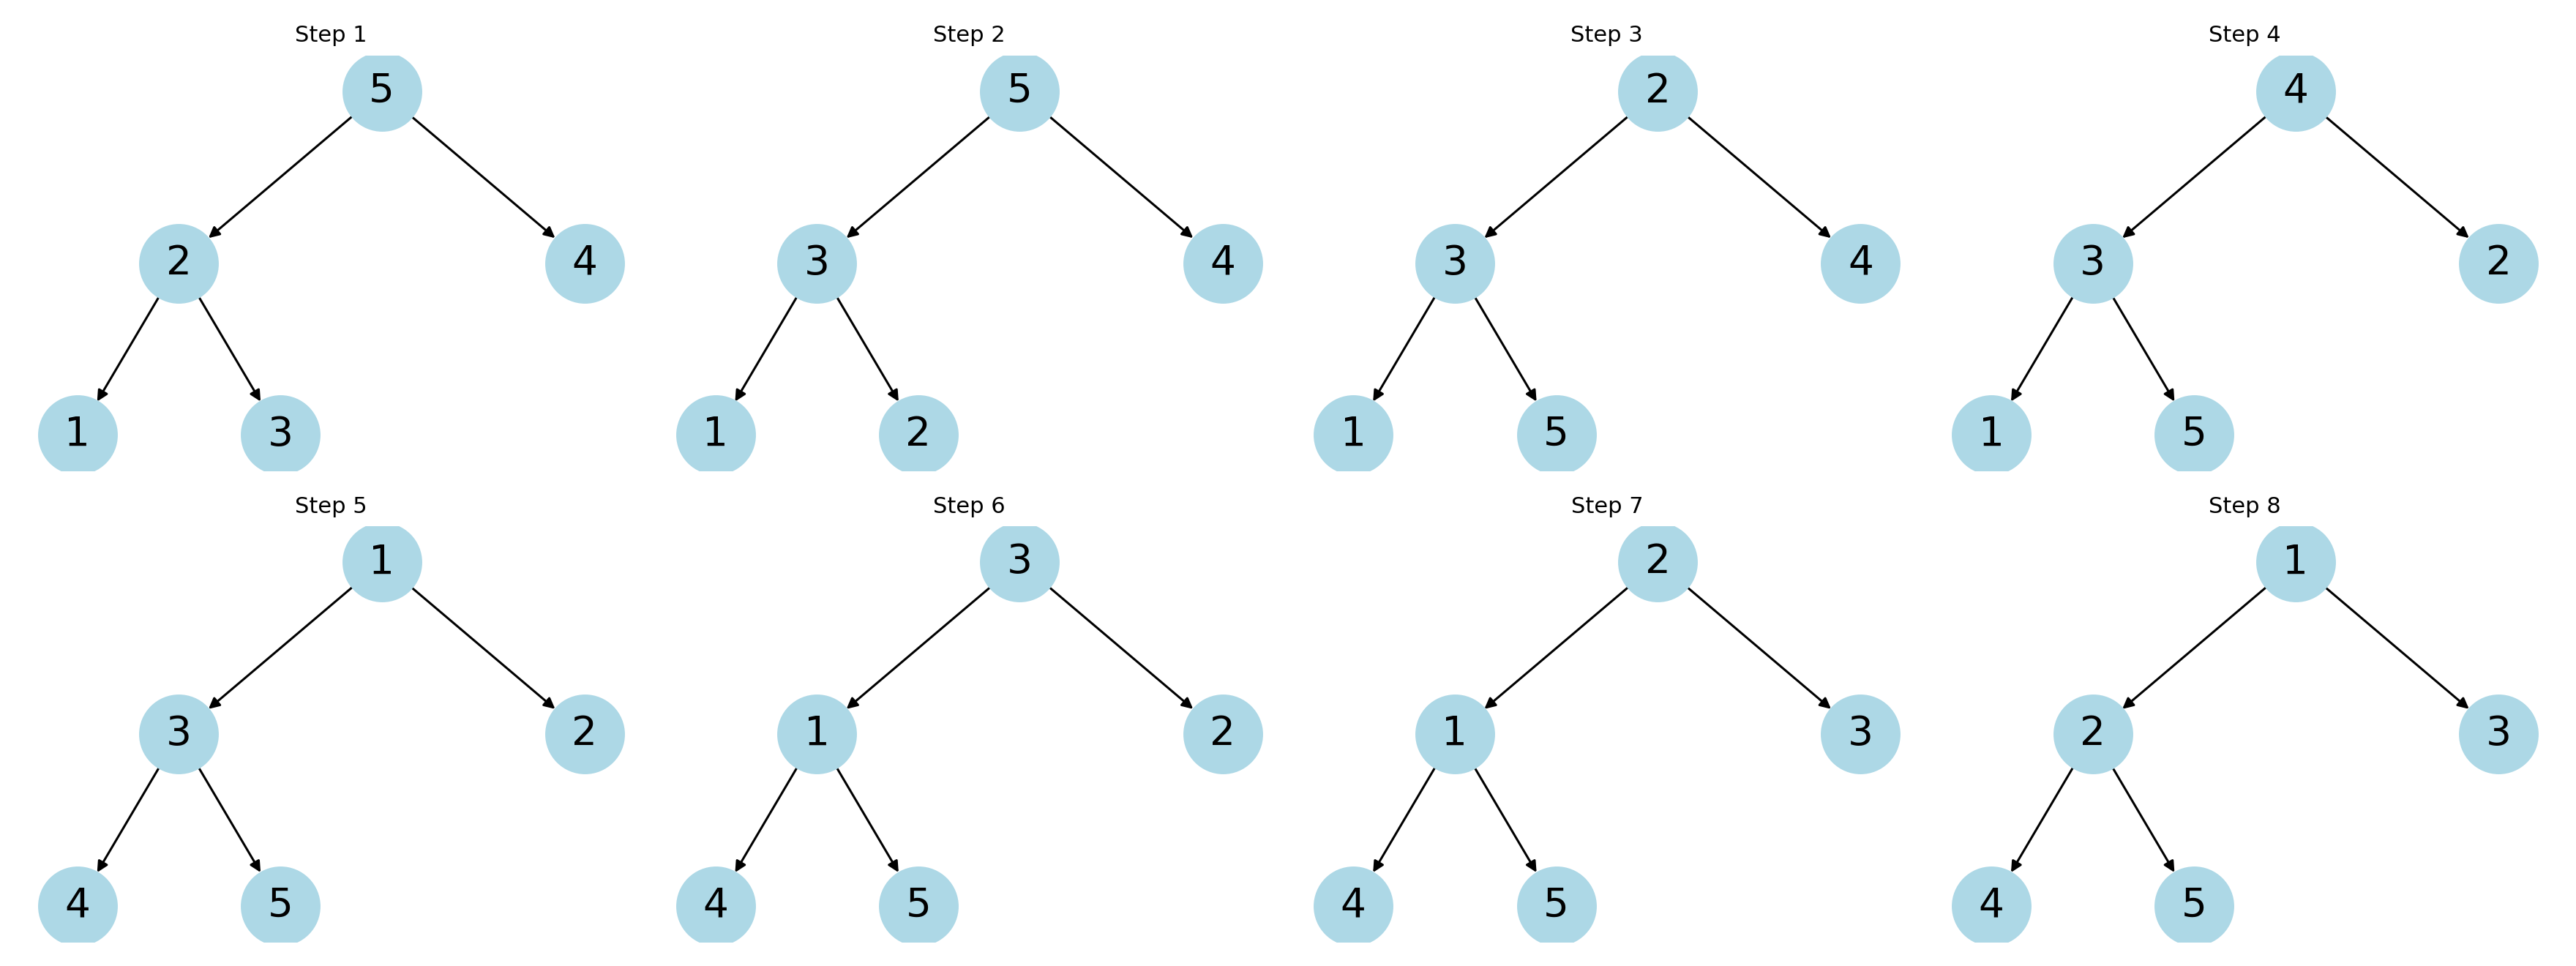
\includegraphics[width=1.1\linewidth]{graphs/heap_sort_comics.png}
\end{frame}

% 17 Heap Sort Animation
\begin{frame}{Heap Sort Animation}
  \vspace*{-2cm}
  \centering
  % 8 fps, frames 000–060
  \animategraphics[autoplay,loop,width=.8\linewidth]{2}{graphs/heapFrame}{000}{060}
\end{frame}

\begin{frame}{Empirical Results ($n=100$, average over 100 runs)}
  \begin{table}[ht]
  \begin{tabular}{l c c}
    \toprule
    Algorithm & Average Swaps & Peak Mem (bytes) \\
    \midrule
    Bubble    & 2469 & 12132593 \\
    Insertion & 388 & 335898 \\
    Merge     & 580  & 502194 \\
    Quick     & 2547  & 2199561 \\
    Heap      & 672  & 583718  \\
    \bottomrule
  \end{tabular}
  \end{table}
\end{frame}

% 20 Runtime Graphs
\begin{frame}{}
    \vspace*{-2cm}
  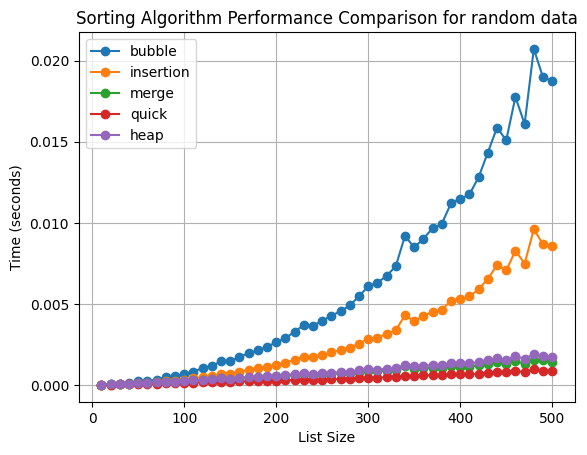
\includegraphics[height=1.3\textheight]{graphs/random.png}\\
\end{frame}

\begin{frame}{}
  \vspace*{-2cm}
  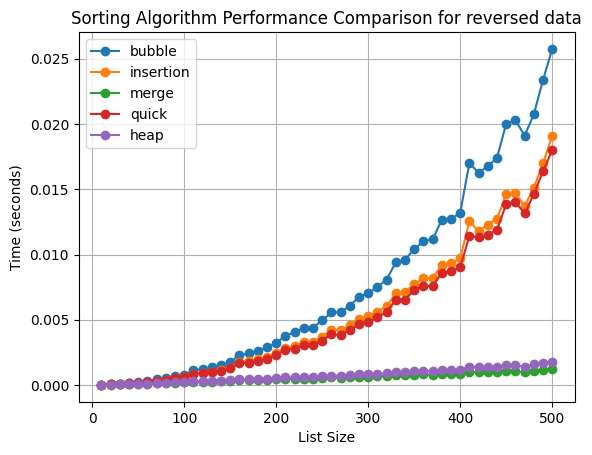
\includegraphics[height=1.3\textheight]{graphs/reversed.png}\\\
\end{frame}

\begin{frame}{}
  \vspace*{-2cm}
  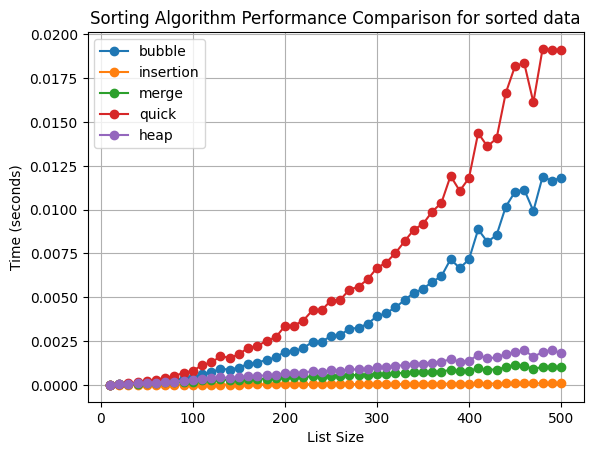
\includegraphics[height=1.3\textheight]{graphs/sorted.png}
\end{frame}

% 21 Memory Usage Graphs
\begin{frame}{}
  \vspace*{-2cm}
  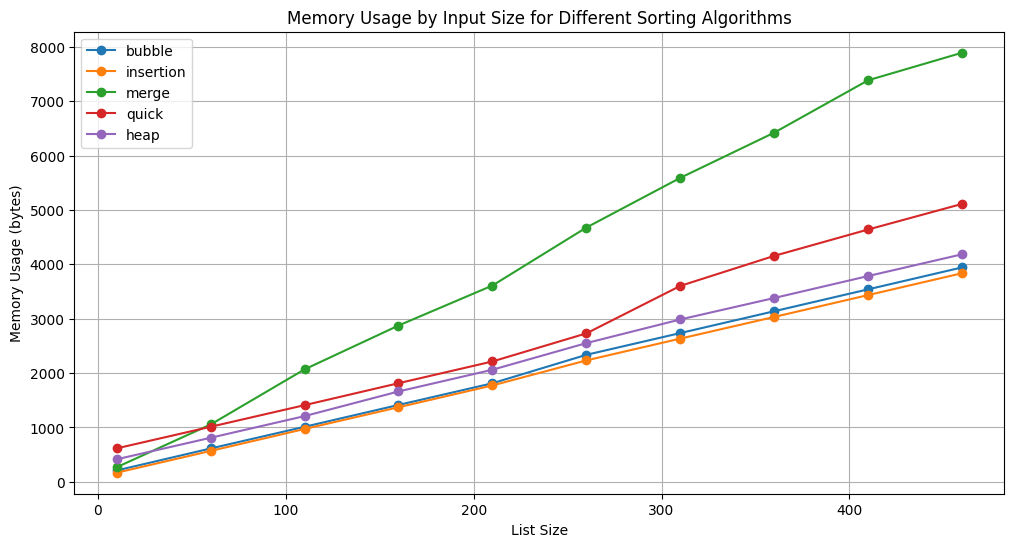
\includegraphics[width=\textwidth]{graphs/memory.png}
\end{frame}

\begin{frame}{Conclusion}
\begin{itemize}
\item Bubble sort and insertion sort are simpler but slower (O(n²))
\item Merge sort, quick sort, and heap sort are faster (O(n log n))
\item Merge sort performs stable on all inputs but Merge Sort may require additional space
\item Quick sort can have problems with already sorted lists
\item Different algorithms perform better on different types of input\\
Choosing an algorithm depends on input size, memory budget, and requirements such as stability or in-place operation.

\end{itemize}
\end{frame}

% 22 Future Research Topics
\begin{frame}{Future Research Topics}
  \begin{itemize}
    \item Parallel and distributed sorting algorithms
    \item External-memory and cache-aware sorts
    \item Cryptographic shuffles and secure permutation generation
  \end{itemize}
\end{frame}

\end{document}
